\documentclass{standalone}
%% Show/hide steps for standalone work — edit this line:
\makeatletter\AtBeginDocument{\@buildstepset{1,2,3,4,5,6,7,8,9,10}}\makeatother
\usepackage{tikz}
\usetikzlibrary{intersections,calc}
\usepackage{amsmath}
\usepackage{hsbcommon}
\begin{document}
    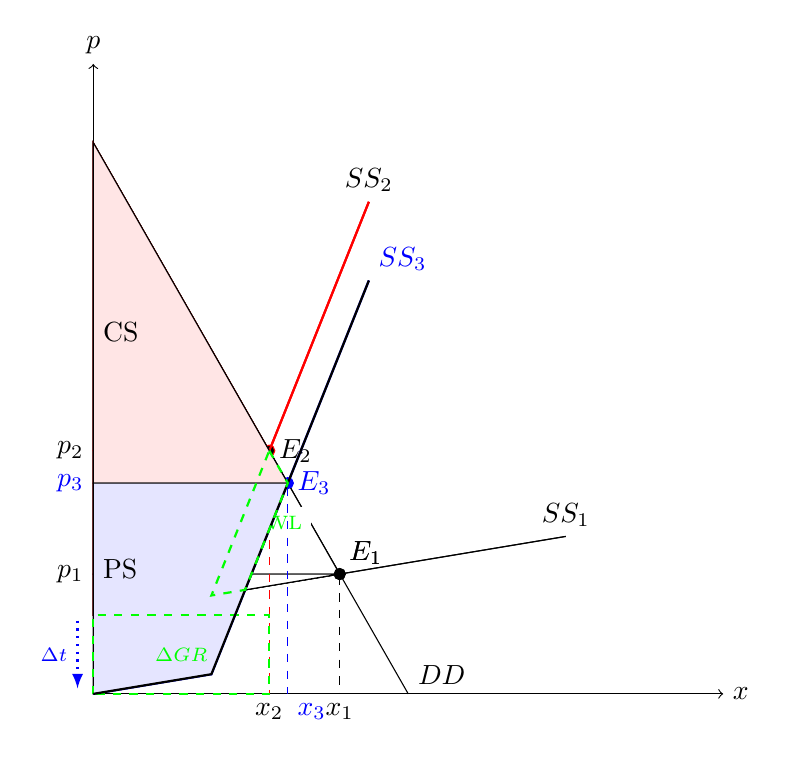
\begin{tikzpicture}
        \draw[->] (0,0) node[below] {\phantom{$X_mi$}} -- (8,0) node (Y) [right] {$x$};
        \draw[->] (0,0) node[left] {\phantom{$Y_mi$}} -- (0,8) node (i) [above] {$p$};

        
        
        \coordinate (A) at (0,7);
        \coordinate (B) at (4,0);
        \coordinate (E) at (0,1);
        \coordinate (F) at (6,2);
        
        \draw[name path=demand] plot [smooth] coordinates {(A) (B) };
        \node[above right] at (B) {$DD$};
        
        \draw[name path=supply] plot [smooth] coordinates {(E) (F)};
        \draw[name path global=oldsupply] plot [smooth] coordinates {(E) (F)};
        \node[above] at (F) {$SS_1$};
            
        \path [name intersections={of=demand and supply,by=X}];
        
        \draw[dashed] (0, |- X) node [left] {$p_1$} -- (X) -- (X |-, 0)  node [below] {$x_1$}; 
        
        \draw[fill=red!10] (A) --  (X) --   (0, |- X) -- node[below right] {\parbox{13ex}{CS}} cycle;
        \draw[fill=blue!10] (E) --  (X) --   (0, |- X) -- node[above right] {\parbox{13ex}{PS}} cycle;
    
        \filldraw (X) node[above right] {$E_1$} circle (2pt);
         \coordinate (Xalt) at (X);
    \ifstep{2}{
\begin{scope}[draw=red]



        \draw[color=black,fill=white] (A) --  (X) --   (0, |- X) --  cycle;
        \draw[color=black,fill=white] (E) --  (X) --   (0, |- X) -- cycle;   
        \filldraw[black] (X) node[above right] {$E_1$} circle (2pt);
        
        \path (E) ++ (1.5,0.25) coordinate (E1);
        \path (E1) ++ (2,5) coordinate (F);
        


        
        \draw[name path=supply,thick] plot coordinates {(E) (E1) (F)};
        \node[above] at (F) {$SS_2$};
            
        % \filldraw[black] (X) node[above right] {$E_1$} circle (2pt);
        
        \path [name intersections={of=demand and supply,by=X}];

        
        \draw[dashed] (0, |- X) node [left] {$p_2$} -- (X) -- (X |-, 0)  node [below] {$x_2$}; 
        
        \draw[fill=red!10] (A) --  (X) --   (0, |- X) -- node[below right] {\parbox{13ex}{CS}} cycle;
        \draw[fill=blue!10] (E) -- (E1)--  (X) --   (0, |- X) -- node[above right] {\parbox{13ex}{PS}} cycle;
    
        \filldraw (X) node[right] {$E_2$} circle (2pt);
        \coordinate (Xalt) at (X);
     
    \end{scope}
}


    \ifstep{3}{
\begin{scope}[color=green]

        \draw (X) -- (Xalt) -- (E1) --  node[fill=white,right] {\scriptsize DWL} cycle;
        \draw[color=red, name path=supply,thick] plot coordinates {(E) (E1) (F)};
    \end{scope}
}


    \ifstep{4}{
\begin{scope}[color=blue]


        % \draw[color=black,fill=white] (A) --  (X) --   (0, |- X) --  cycle;
        % \draw[color=black,fill=white] (E) --  (X) --   (0, |- X) -- cycle;   
        
        \path (E) ++ (0,-1) coordinate (E2);
        \path (E1) ++ (0,-1) coordinate (E12);
        \path (F) ++ (0,-1) coordinate (F2);

        \draw[->,>=latex,shorten >=2pt, shorten <=2pt,thick,dotted] (E) ++ (-0.2,0) -- node[left] {\scriptsize $\Delta t$}  ++ (0,-1);
        
       
        \draw[name path global=supply,thick] plot coordinates {(E2) (E12) (F2)};
        \node[above right] at (F2) {$SS_3$};
            
        % \filldraw[black] (X) node[above right] {$E_1$} circle (2pt);
        
        \path [name intersections={of=demand and supply,by=X}];

        
        \draw[dashed] (0, |- X) node [left] {$p_3$} -- (X) -- (X |-, 0)  node [below right] {$x_3$}; 
        
    
        \filldraw (X) node[right] {$E_3$} circle (2pt);


    \end{scope}
}

            
    \ifstep{5}{

        
        
        \draw[fill=red!10] (A) --  (X) --   (0, |- X) -- node[below right] {\parbox{13ex}{CS}} cycle;
        \draw[fill=blue!10] (E2) -- (E12)--  (X) --   (0, |- X) -- node[above right] {\parbox{13ex}{PS}} cycle;
        \draw[dashed, green, thick] (0,0) rectangle node {\scriptsize $\Delta GR$} (Xalt |-, 1);

        \draw[name path global=supply,thick] plot coordinates {(E2) (E12) (F2)};

        \path [name intersections={of=oldsupply and supply,by=LA}];
        \draw[dashed, color=green,thick] (Xalt) -- (X) -- (LA) -- (E1) -- cycle;

        % \filldraw[red] (LA) circle (4pt);
        
    }

    \end{tikzpicture}
\end{document}